\documentclass[12pt]{article}

\usepackage[margin=1in]{geometry}  % set the margins to 1in on all sides
\usepackage{graphicx}              % to include figures
\usepackage{amsmath}               % great math stuff
\usepackage{amsfonts}              % for blackboard bold, etc
\usepackage{amsthm}                % better theorem environments
\usepackage{url}

% various theorems, numbered by section

\newtheorem{thm}{Theorem}[section]
\newtheorem{lem}[thm]{Lemma}
\newtheorem{prop}[thm]{Proposition}
\newtheorem{cor}[thm]{Corollary}
\newtheorem{conj}[thm]{Conjecture}

\DeclareMathOperator{\id}{id}

\newcommand{\bd}[1]{\mathbf{#1}}  % for bolding symbols
\newcommand{\RR}{\mathbb{R}}      % for Real numbers
\newcommand{\ZZ}{\mathbb{Z}}      % for Integers
\newcommand{\col}[1]{\left[\begin{matrix} #1 \end{matrix} \right]}
\newcommand{\comb}[2]{\binom{#1^2 + #2^2}{#1+#2}}
	

\begin{document}


\nocite{*}

\title{A Generalized Sphere Theorem for Positively Curved Combinatorial 3-Manifolds}

\author{Aaron Trout \\ Department of Mathematics \\
Chatham University \\ Woodland Rd, Pittsburgh PA 15232 USA \and
Vadas Gintautas\\ Department of Physics \\
Chatham University \\ Woodland Rd, Pittsburgh PA 15232 USA}


\maketitle

\begin{abstract}
  This paper presents a discrete version of Grove and Shiohama's generalized sphere theorem \cite{groveshiohama}.
\end{abstract}


\section{Introduction}

Differential geometry is of central importance not only to geometers but also topologists, physicists and, increasingly, many of those interested in applied topics such as finite element analysis REFERENCE and computer graphics REFERENCE. One new offshoot in this area is {\em discrete differential geometry} (DDG) which seeks discrete analogs to the classical theorems and concepts from differential geometry. Since many way computational treatments of differential geometry involve discretizing shapes, this subject has particular relevance for those with applied interests REFERECE. Other recent DDG work can be found in \cite{BMM,Crowley,EMM,forman2,GGL1,GGL2,GGL3,LS,stone}. 

A particularly important goal in classical differential geometry is to elucidate the relationship between the curvature of a Riemannian (or semi-Riemannian) space and its topology. The classical
results in this area are numerous, beautiful, and have inspired an
enormous amount of subsequent research (REFERENCES). In this paper, we will present a discrete analog of the ``generalized'' sphere theorem of Grove and Shiohama \cite{groveshiohama}.

\begin{thm}[Grove-Shiohama] Let $M$ be a complete, connected, $n$-dimensional Riemannian manifold with section curvature $K \geq \delta > 0$ and $diam(M) > \frac{\pi}{2\sqrt{\delta}}$. Then, $M$ is homeomorphic to a sphere.
\end{thm}

\noindent Note that the diameter bound in this theorem is exacly half that allowed by the Bonnet-Myers theorem:

\begin{thm}[Bonnet-Myers] Let $M$ be a complete, connected, $n$-dimensional Riemannian manifold with section curvature $K \geq \delta > 0$. Then $diam(M) \leq \frac{\pi}{\sqrt{\delta}}$.
\end{thm}

\section{Basic Stuff}
\label{sect:basics}

\begin{figure}
    \begin{center}
        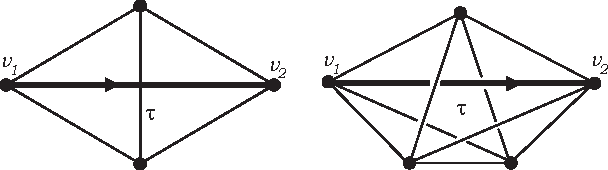
\includegraphics[width=0.6\linewidth]{figures/hops.pdf}
        \caption{Hop diagram}
    \end{center}
\end{figure}


\begin{figure}
    \begin{center}
        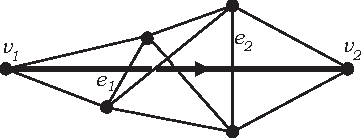
\includegraphics[width=0.6\linewidth]{figures/jump.pdf}
        \caption{Jump diagram}
    \end{center}
\end{figure}
\section{Results}

diameter statistics by topological type

\begin{tabular} {| l l | l l | l l | l l | l l |}
\hline
\multicolumn{2}{|c|}{$S^{3}/Q$} &
\multicolumn{2}{|c|}{$L(3,1)$} &
\multicolumn{2}{|c|}{$RP^{3}$} &
\multicolumn{2}{|c|}{$S^{3}$} &
\multicolumn{2}{|c|}{$L(4,1)$} \\
\hline
\hline
$1H$&1    &$2E$&1    &$1H$&10    &$1E$&3    &$1J$&1 \\
  &       &$1J$&1    &$2E$&7     &$1H$&173  &    &  \\
  &       &  &       &$1J$&5     &$2E$&401  &    &  \\
  &       &  &       &    &      &$1J$&2438 &    &  \\
  &       &  &       &    &      &$3E$&1060 &    &  \\
  &       &  &       &    &      &$2H$&582  &    &  \\
  &       &  &       &    &      &$4E$&93   &    &  \\
  &       &  &       &    &      &$2J$&11   &    &  \\
\hline
\end{tabular}

global diameter statistics by topological type

\begin{tabular} {| l l |}
\hline
$1E$ &       3\\
$1H$ &       184\\
$2E$ &       409\\
$1J$ &       2445\\
$3E$ &       1060\\
$2H$ &       582\\
$4E$ &       93\\
$2J$ &       11\\
\hline
\end{tabular}


\begin{figure}
    \begin{center}
    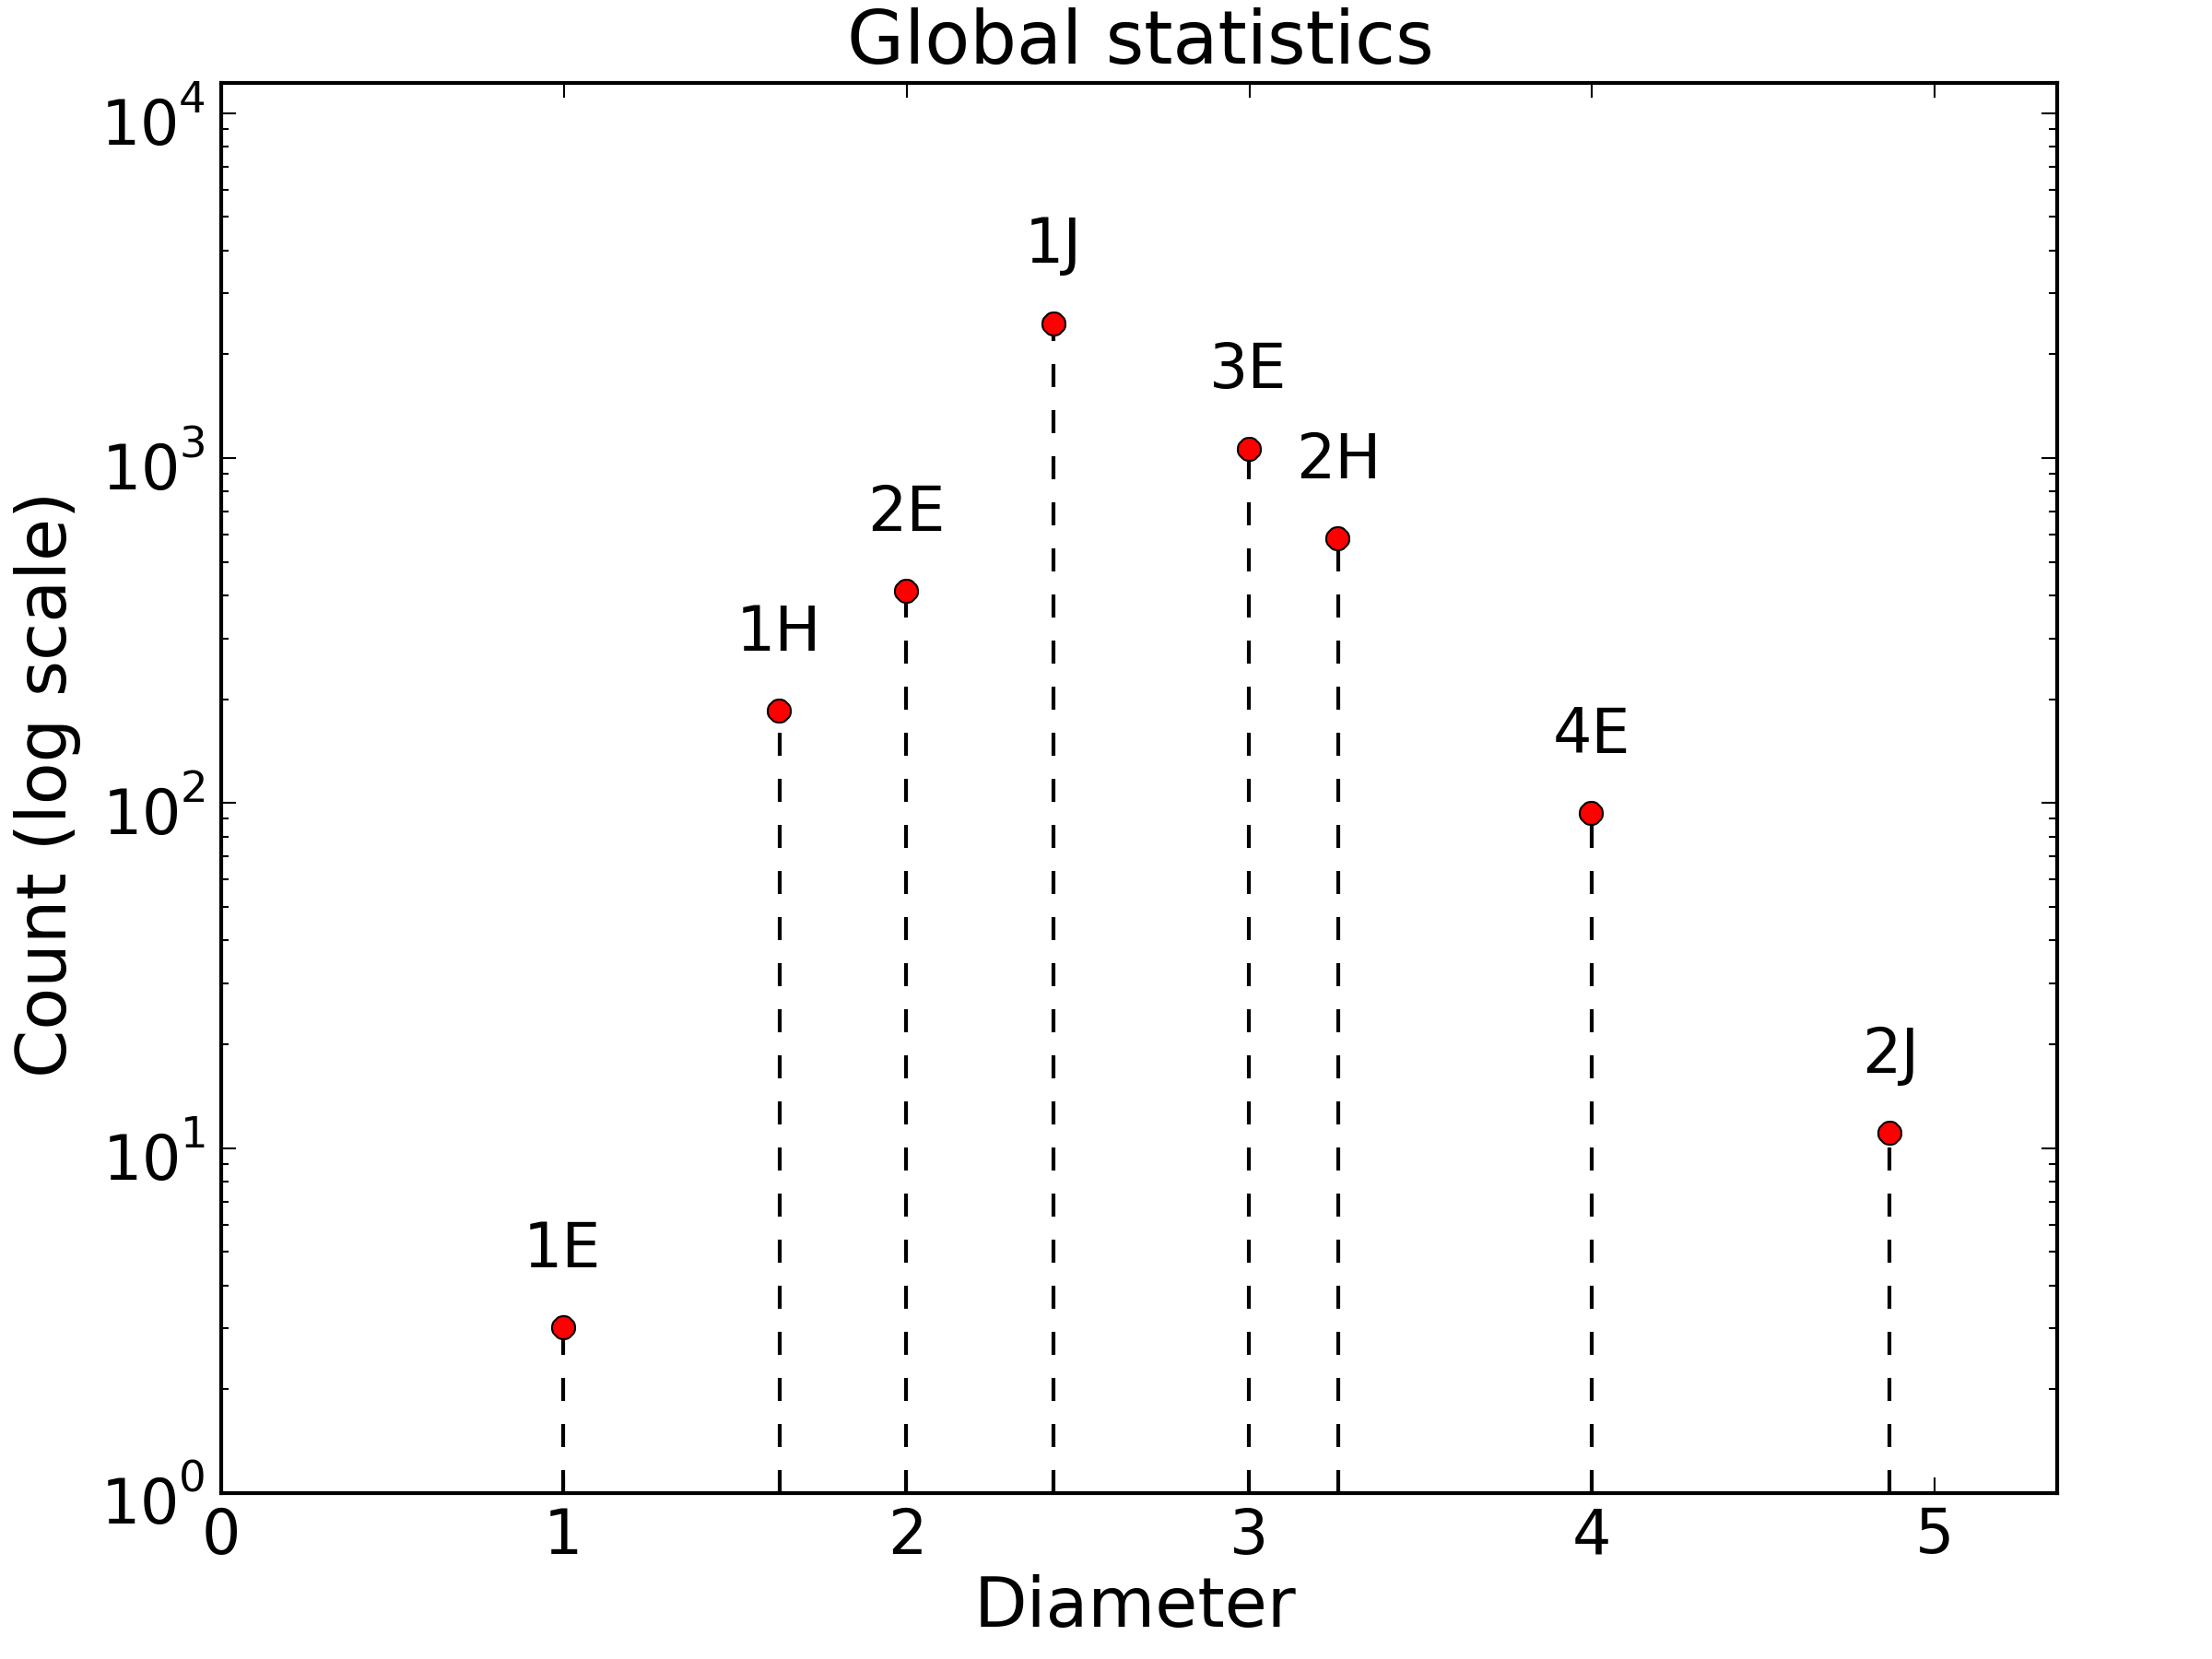
\includegraphics[width=0.6\linewidth]{figures/global_statistics.png}
    \caption{Global statistics}
    \end{center}
\end{figure}

\bibliographystyle{plain}
\bibliography{manifolds}
\end{document}
